\section{Coupled Results}
\label{sec:coupledResults}

\begin{frame}{Remember why we are here}
  \pause
  \huge Model a nuclear reactor.
\end{frame}

\begin{frame}{Advanced Burner Reactor Benchmark}
  \begin{itemize}
    \item Benchmark published February 2016 \cite{abr}.
    \item Four designs including MET-1000.
    \item Thirty-one solutions including \dif.
  \end{itemize}
\end{frame}

\begin{frame}{MET-1000}
  \begin{itemize}
    \item Eighteen cross-section regions.
    \item Forty-Nine material compositions.
    \item Dimensions and isotopic compositions fully specified.
  \end{itemize}
  \vspace{0.2in}
  \begin{itemize}
    \item Cross-sections generated independently.
    \item Dimensions \textit{appear} thermally expanded.
  \end{itemize}
\end{frame}

\begin{frame}{RESULTS ARE WRONG!}
  \begin{itemize}
    \item This chapter isn't written yet.
    \item I know the results in this section are wrong.
    \item Still working on the model, but I have the scripts to generate these
      plots.
    \item Please look at the ideas, not the numbers.
  \end{itemize}
\end{frame}

\begin{frame}{Reactivity Coefficients}
  Define the following reactivity coefficients 
  $\alpha_{Total}$\\
  $\alpha_{T_{\!\mbox{\scriptsize \em exp}}}$\\
  $\alpha_{T_{exp}}$\\
  $\alpha_{CTC}$\\ % (coolant temperature coefficient)
  $\alpha_{Doppler}$
\end{frame}

\begin{frame}{Eigenvalue Result}
  \vspace{-0.25in}
  \begin{figure}
    \centering
    \subfloat[$\phi_{1}$]{
      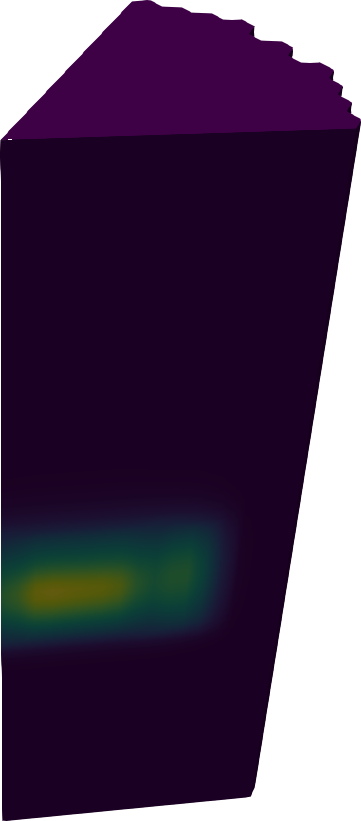
\includegraphics[width=0.25\textwidth]{./figs/phi_nod_group1}}
    \hspace{1in}
    \subfloat[$\phi_{33}$]{
      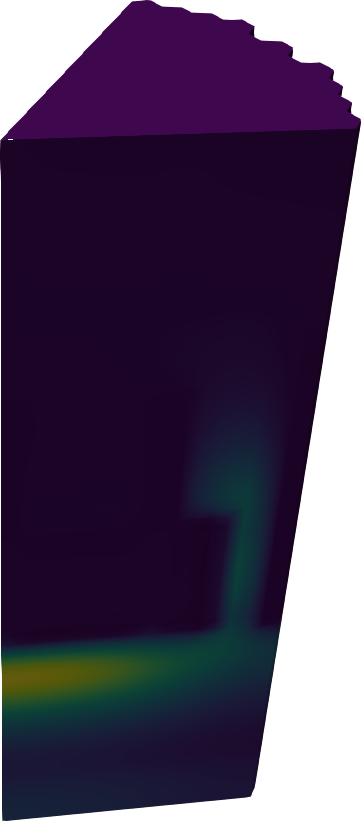
\includegraphics[width=0.25\textwidth]{./figs/phi_nod_group33}}
  \end{figure}
  \begin{block}{}
    $\keff = X.XXXXXX \qquad (+XXX \units{pcm})$ expected $\pm 600\units{pcm}$
  \end{block}
\end{frame}

\begin{frame}{Power Feedback}
  \begin{figure}
    \centering
    \subfloat{
      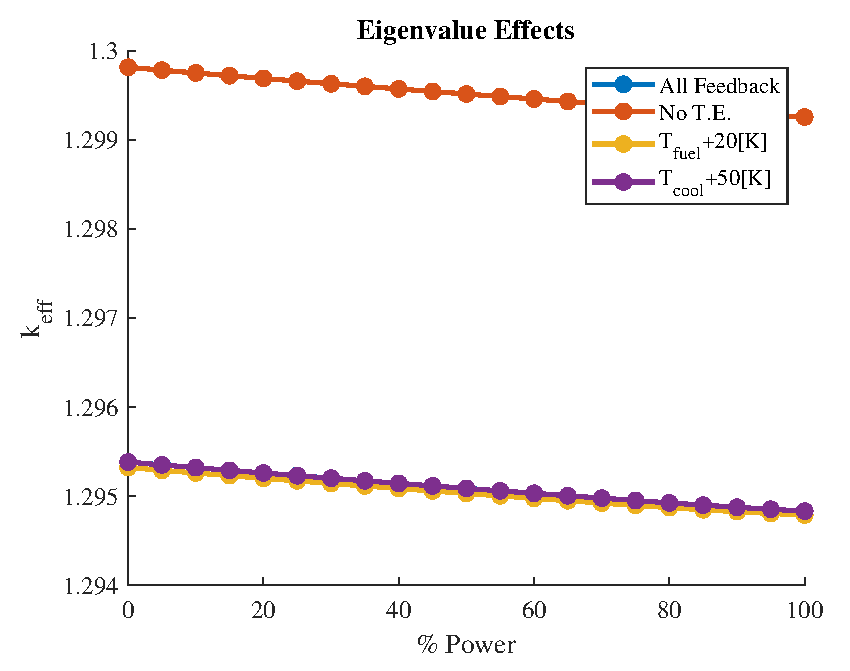
\includegraphics[width=0.5\textwidth]{eigenvalue_effects}}
    \hspace*{\fill}
    \subfloat{
      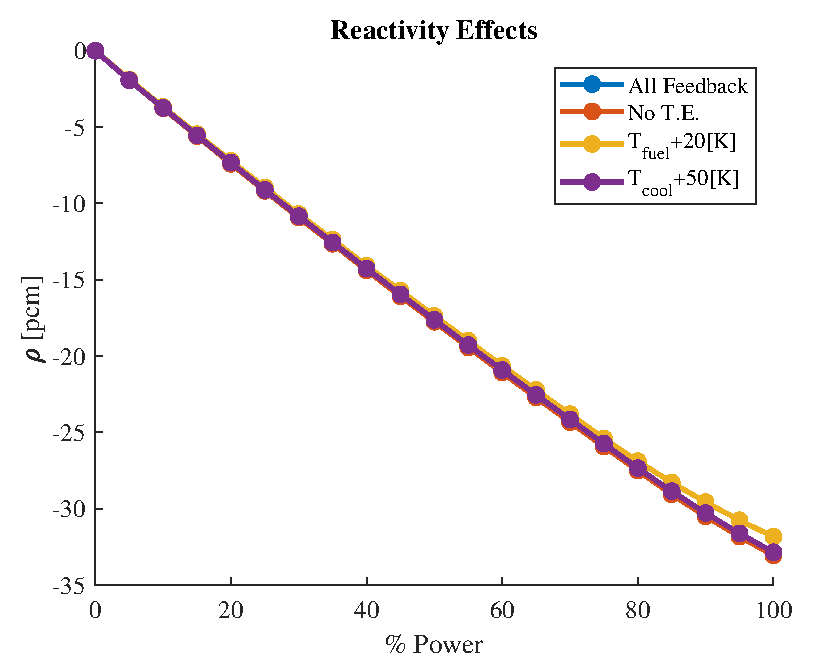
\includegraphics[width=0.5\textwidth]{reactivity_effects}}
  \end{figure}
\end{frame}

\begin{frame}{Reactivity Coefficients}
  \begin{figure}
    \centering
    \subfloat{
      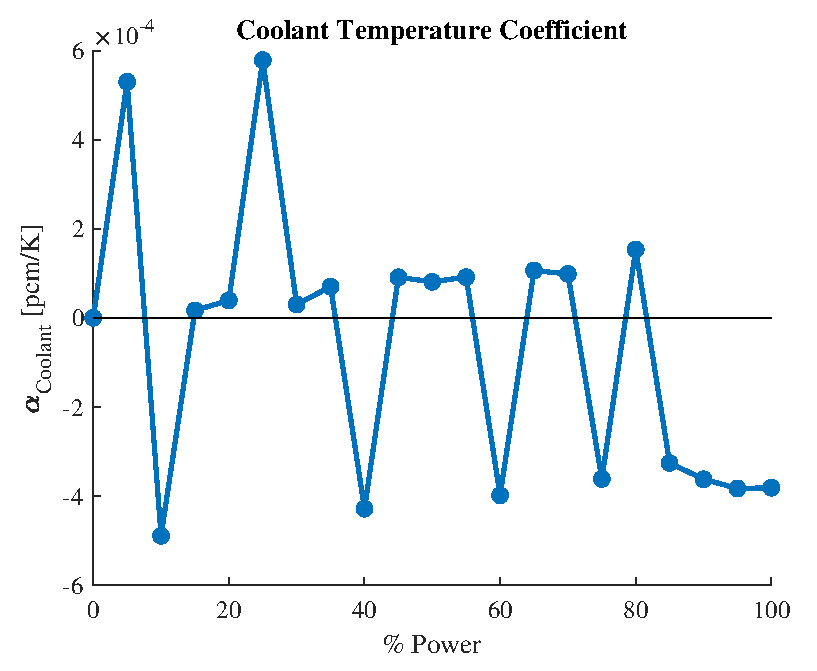
\includegraphics[width=0.5\textwidth]{alpha_ctc}}
    \hspace*{\fill}
    \subfloat{
      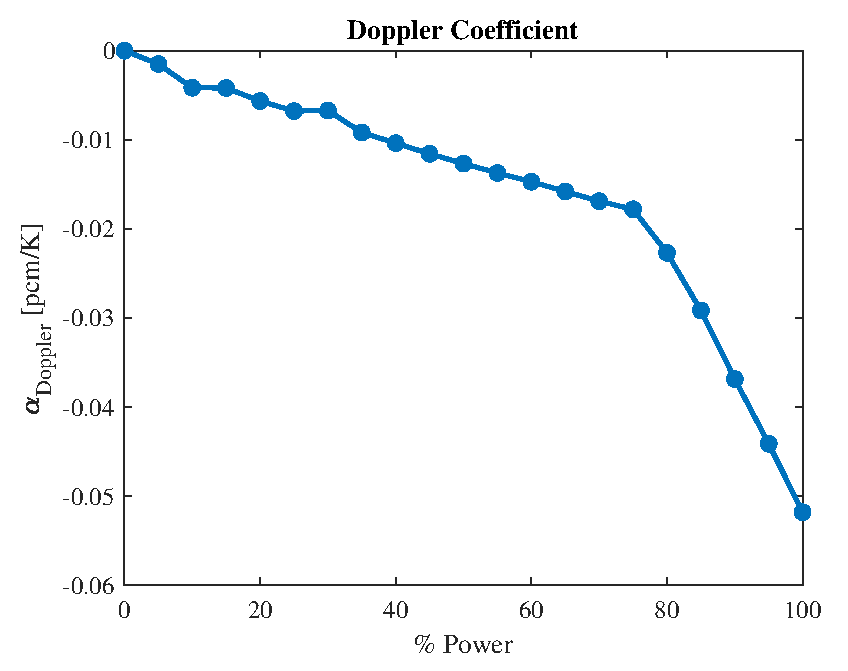
\includegraphics[width=0.5\textwidth]{alpha_doppler}}
  \end{figure}
\end{frame}
